\documentclass[border=3pt]{standalone}
\usepackage{mathptmx}
\usepackage{tikz}
\usetikzlibrary{positioning,arrows.meta,fit,calc}
\begin{document}
\small\hyphenpenalty=10000\exhyphenpenalty=10000
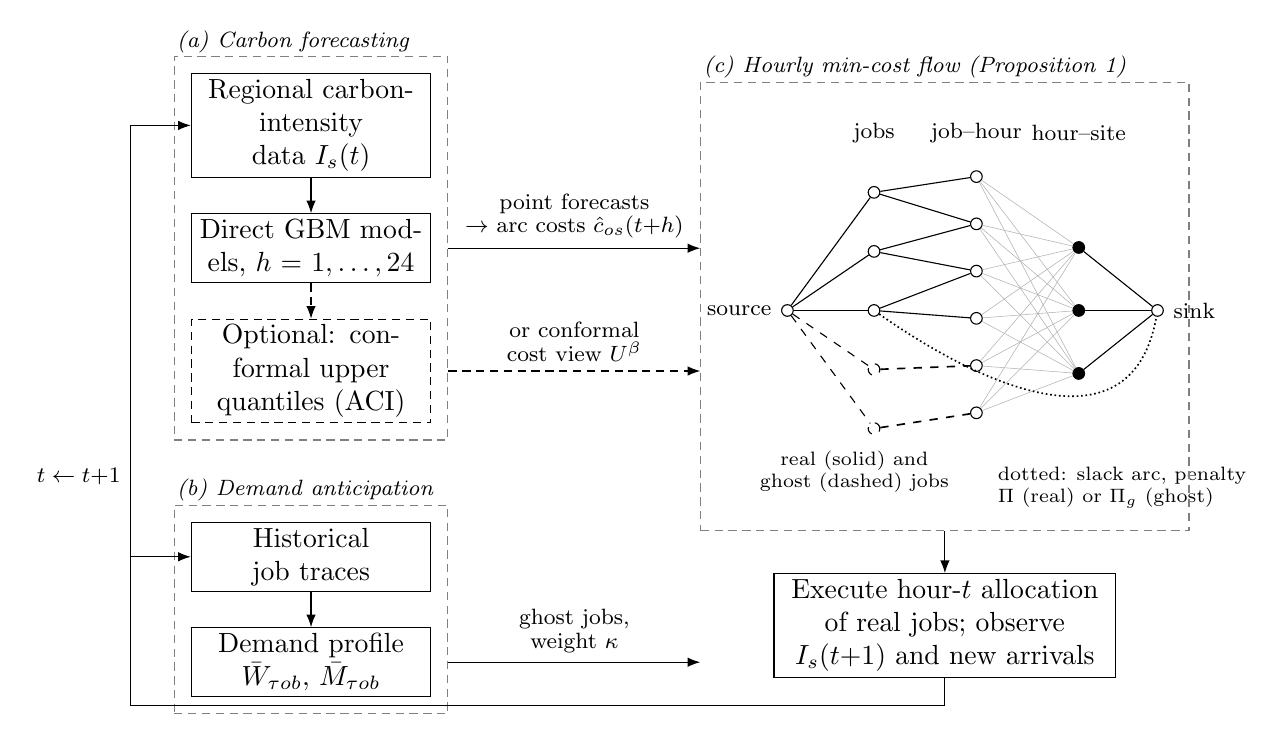
\begin{tikzpicture}[
  blk/.style={draw,thin,minimum height=0.8cm,text width=2.9cm,align=center,inner sep=2pt},
  frm/.style={draw,densely dashed,gray,inner sep=6pt},
  lab/.style={font=\footnotesize\itshape,anchor=south west,inner sep=1pt},
  ar/.style={-{Latex[length=1.6mm,width=1.2mm]},thin},
  nd/.style={circle,draw,thin,fill=white,inner sep=0pt,minimum size=4.2pt}]
% ---- forecasting module
\node[blk] (feed) at (0,0) {Regional carbon-intensity data $I_s(t)$};
\node[blk,below=0.45cm of feed] (gbm) {Direct GBM models, $h=1,\dots,24$};
\node[blk,below=0.45cm of gbm,densely dashed] (cp) {Optional: conformal upper quantiles (ACI)};
\draw[ar] (feed)--(gbm); \draw[ar,densely dashed] (gbm)--(cp);
\node[frm,fit=(feed)(cp)] (F1) {};
\node[lab] at (F1.north west) {(a) Carbon forecasting};
% ---- demand module
\node[blk,below=1.25cm of cp] (hist) {Historical job traces};
\node[blk,below=0.45cm of hist] (prof) {Demand profile $\bar W_{\tau ob},\,\bar M_{\tau ob}$};
\draw[ar] (hist)--(prof);
\node[frm,fit=(hist)(prof)] (F2) {};
\node[lab] at (F2.north west) {(b) Demand anticipation};
% ---- planning network
\begin{scope}[shift={(8.25,-2.35)}]
 \node[nd,label={[font=\footnotesize]left:source}] (s) at (-2.2,0) {};
 \foreach \y/\n in {1.5/1,0.75/2,0/3}{\node[nd] (j\n) at (-1.1,\y) {};}
 \foreach \y/\n in {-0.75/4,-1.5/5}{\node[nd,dashed] (j\n) at (-1.1,\y) {};}
 \foreach \y/\n in {1.7/1,1.1/2,0.5/3,-0.1/4,-0.7/5,-1.3/6}{\node[nd] (h\n) at (0.2,\y) {};}
 \foreach \y/\n in {0.8/1,0.0/2,-0.8/3}{\node[nd,fill=black] (k\n) at (1.5,\y) {};}
 \node[nd,label={[font=\footnotesize]right:sink}] (t) at (2.5,0) {};
 \foreach \n in {1,2,3}{\draw[thin] (s)--(j\n);}
 \foreach \n in {4,5}{\draw[thin,dashed] (s)--(j\n);}
 \draw[thin] (j1)--(h1) (j1)--(h2) (j2)--(h2) (j2)--(h3) (j3)--(h3) (j3)--(h4);
 \draw[semithick,dashed] (j4)--(h5) (j5)--(h6);
 \foreach \a in {1,...,6}{\foreach \b in {1,2,3}{\draw[very thin,gray!60] (h\a)--(k\b);}}
 \foreach \b in {1,2,3}{\draw[thin] (k\b)--(t);}
 \draw[semithick,densely dotted] (j3) to[out=-35,in=-100,looseness=1.25] (t);
 \node[font=\scriptsize,align=left,anchor=west] at (0.35,-2.25) {dotted: slack arc, penalty\\ $\Pi$ (real) or $\Pi_g$ (ghost)};
 \node[font=\footnotesize,align=center] at (-1.1,2.25) {jobs};
 \node[font=\footnotesize,align=center] at (0.2,2.25) {job--hour};
 \node[font=\footnotesize,align=center] at (1.5,2.25) {hour--site};
 \node[font=\scriptsize,align=center] at (-1.35,-2.05) {real (solid) and\\ ghost (dashed) jobs};
 \node[font=\scriptsize,gray] at (0.85,-2.25) {};
\end{scope}
\node[frm,minimum width=6.2cm,minimum height=5.7cm] (F3) at (8.05,-2.3) {};
\node[lab] at (F3.north west) {(c) Hourly min-cost flow (Proposition 1)};
% ---- execution
\node[blk,text width=4.2cm] (exe) at (8.05,-6.35) {Execute hour-$t$ allocation of real jobs; observe $I_s(t{+}1)$ and new arrivals};
% ---- connections
\draw[ar] (gbm.east -| F1.east) -- node[above,font=\footnotesize,align=center]{point forecasts\\[-1pt] $\to$ arc costs $\hat c_{os}(t{+}h)$} (gbm.east -| F3.west);
\draw[ar,densely dashed] (cp.east -| F1.east) -- node[above,font=\footnotesize,align=center]{or conformal\\[-1pt] cost view $U^{\beta}$} (cp.east -| F3.west);
\draw[ar] (prof.east -| F2.east) -- node[above,font=\footnotesize,align=center]{ghost jobs,\\[-1pt] weight $\kappa$} (prof.east -| F3.west);
\draw[ar] (F3.south) -- (exe.north);
\draw[ar] (exe.south) -- ++(0,-0.35) -| node[pos=0.75,left,font=\footnotesize]{$t\leftarrow t{+}1$} ([xshift=-0.55cm]F1.west) |- (feed.west);
\draw[ar] ([xshift=-0.55cm]F2.west |- hist.west) -- (hist.west);
\end{tikzpicture}
\end{document}
